%-------------------------------------------------------------------------------
% This file provides a skeleton ATLAS document.
%-------------------------------------------------------------------------------
% Specify where ATLAS LaTeX style files can be found.
\newcommand*{\ATLASLATEXPATH}{latex/}
% Use this variant if the files are in a central location, e.g. $HOME/texmf.
% \newcommand*{\ATLASLATEXPATH}{}
%-------------------------------------------------------------------------------
\documentclass[UKenglish,texlive=2013]{\ATLASLATEXPATH atlasdoc}
% The following command is needed by arXiv to ensure use of pdflatex.
% It should be included in the first 5 lines of the preamble.
% \pdfoutput=1
% The language of the document must be set: usually UKenglish or USenglish.
% british and american also work!
% Commonly used options:
%  texlive=YYYY          Specify TeX Live version (2013 is default).
%  atlasstyle=true|false Use ATLAS style for document (default).
%  coverpage             Create ATLAS draft cover page for collaboration circulation.
%                        See atlas-draft-cover.tex for a list of variables that should be defined.
%  cernpreprint          Create front page for a CERN preprint.
%                        See atlas-preprint-cover.tex for a list of variables that should be defined.
%  PAPER                 The document is an ATLAS paper (draft).
%  CONF                  The document is a CONF note (draft).
%  PUB                   The document is a PUB note (draft).
%  txfonts=true|false    Use txfonts rather than the default newtx - needed for arXiv submission.
%  paper=a4|letter       Set paper size to A4 (default) or letter.

%-------------------------------------------------------------------------------
% Extra packages:
\usepackage{\ATLASLATEXPATH atlaspackage}
% Commonly used options:
%biblatex=false|true   Use biblatex (default) or bibtex for the bibliography.
%  backend=biber         Use the biber backend rather than bibtex.
%  subfigure|subfig|subcaption  to use one of these packages for figures in figures.
%  minimal               Minimal set of packages.
%  default               Standard set of packages.
%  full                  Full set of packages.
%-------------------------------------------------------------------------------
% Style file with biblatex options for ATLAS documents.
\usepackage{\ATLASLATEXPATH atlasbiblatex}

% Package for creating list of authors and contributors to the analysis.
\usepackage{\ATLASLATEXPATH atlascontribute}

% Useful macros
\usepackage{\ATLASLATEXPATH atlasphysics}
\usepackage{comment}
% See doc/atlas-physics.pdf for a list of the defined symbols.
% Default options are:
%   true:  journal, misc, particle, unit, xref
%   false: BSM, hion, math, process, other, texmf
% See the package for details on the options.

% Files with references for use with biblatex.
% Note that biber gives an error if it finds empty bib files.
\addbibresource{LaserII_note.bib}
%\addbibresource{bibtex/bib/ATLAS.bib}

% Paths for figures - do not forget the / at the end of the directory name.
\graphicspath{{logos/}{figures/}}

% Add you own definitions here (file LaserII_note-defs.sty).
%\usepackage{LaserII_note-defs}
\newcommand{\laser}{{\sc LASER}}
\newcommand{\las}{{\sc LASER}}
\newcommand{\lasa}{{\sc LASER~I}}
\newcommand{\lasi}{{\sc LASERI}}
\newcommand{\lasii}{{\sc LASERII}}
\newcommand{\lasb}{{\sc LASER~175}}
\newcommand{\lasc}{{\sc LASER~II}}
\newcommand{\atlas}{{\sc ATLAS}}
\newcommand{\pmts}{{\sc PMTs}}
\newcommand{\pmt}{{\sc PMT}}
\newcommand{\tilecal}{{\sc TILECAL}}
\newcommand{\vme}{{\sc VME}}
\newcommand{\phocal}{{\sc PHOCAL}}
\newcommand{\licphd}{{\sc LICPHD}}
\newcommand{\licpmt}{{\sc LICPMT}}
\newcommand{\licmot}{{\sc LICMOT}}
\newcommand{\lascar}{{\sc LASCAR}}
\newcommand{\polas}{{\sc POLAS}}
\newcommand{\charinjsplit}{{\sc CIS}}
\newcommand{\coimbra}{Co\"{i}mbra}
\newcommand{\mum}{$\mu m$}

%-------------------------------------------------------------------------------
% Generic document information
%-------------------------------------------------------------------------------

% Title, abstract and document 
\input{LASERII_note-metadata}
% Author and title for the PDF file
\hypersetup{pdftitle={Upgrade of the LASER calibration system of the ATLAS Tile Calorimeter},pdfauthor={The ATLAS Collaboration}}

%-------------------------------------------------------------------------------
% Content
%-------------------------------------------------------------------------------
\begin{document}

\maketitle

\tableofcontents

% List of contributors - print here or after the Bibliography.
%\PrintAtlasContribute{0.30}
%\clearpage

%-------------------------------------------------------------------------------
\section{Introduction}
\label{sec:intro}
%-------------------------------------------------------------------------------

The Atlas Tilecal hadronic calorimeter is equipped with a 3-level calibration system to monitor and  calibrate the response of the active devices (plastic scintillating tiles), the response of the PMTs receiving the light from clusters of tiles (cells), and the response of the Front End and digitization electronics of the individual readout channels. \par
The global detector calibration is performed monthly by measuring the individual cell response to a reference excitation produced by calibrated Cesium sources which float inside the detector through a suitable pipe network.
Calibration of the PMTs and of the readout chain are performed between two sucessive Cesium scans; laser pulses are distributed to each individual PMT cathode (approximatively 10,000 channels) by a suitable optical distribution line having a power laser (several $\mu$J per pulse) as a source. Laser calibrations can be performed every two-three days during pauses of LHC collisions and during collision runs by pulsing the laser in the empty bunch intervals.  \par
During the Long Shutdown I of LHC operations, the Tilecal laser calibration system has been re-designed, tested, and installed for the Run II operations. The shortcomings of the optical part have been studied, understood and solved. The LASER light injected in the PMTs is measured by sets of photodiodes at several stages of the optical path. The monitoring of the photodiodes is performed by a redundant internal calibration scheme using an LED, a radioactive source, and a charge injection system. \par
A challenge of the new LASER project lied in the design of electronics boards that would overcome the shortcomings of the previous LASER system (interface with the LHC clock and saturation of the electronics for higher LASER intensities) and that would be compatible with the new requirements (increase of the number of photodiodes, new internal calibration scheme). A new electronics has been designed to achieve these goals.


%-------------------------------------------------------------------------------
\section{The LASERI system during P1: performance and shortcomings}
\label{sec:detector}
%-------------------------------------------------------------------------------

\input LaserI.tex

%-------------------------------------------------------------------------------
\section{The LASERII system}
\label{sec:result}
%-------------------------------------------------------------------------------

\subsection{Overview}

The main concern of the \lasii~project was to design a calibration system without \lasi~shortcomings while maintaining a high performance level in terms of precision and stability. The major improvements are summarized in table \ref{tab:lasii_imp}.
\begin{table*}[!htpb]
 \begin{center}
 \begin{tabular}{|l|l|}
\hline
Critical Point & \lasii \\
\hline
Measurement of the LASER light & Number of photodiodes increased to 10+1 \\
at each point of the optical path & \\
\hline
Adapt the calibration system of the photodiodes & Redundant calibration scheme: \\
& (Light Emitting diode (LED) \\
& and a static radioactive source \\
\hline
Insufficient light mixing of each optical set & New design of the beam expander \\
& (light to the ~400 fibers of the TileCal)  \\
& and of other mixers \\
& (LASER head and filter wheel outputs) \\
\hline
Optics box in a vertical position & Optics box in an horizontal position\\
\hline
Saturation of the photodiode electronics & Dynamic range increased  (13 bits-ADC) \\
\hline
Electronics shortcomings  & new card including all functionnalities \\
(LASTROD memory, LHC clock) & \\
\hline
\end{tabular}
\caption{Critical points of the \lasi~system and improvements in the \lasii}\label{tab:lasii_imp}
\end{center}
\end{table*}
\par
A better estimation of the LASER light injected in the system is possible thanks to an increase of the number of photodiodes. In that case, the calibration scheme of the photodiodes used for the \lasi~(a moving radioactive source) is difficult to use. We thus moved to a system comprised of a Light Emitting Diode (LED) and of a static radioactive source. The LED signal is injected in the ten photodiodes dedicated to the measurement of the LASER light and in a reference photodiode monitored through the static radioactive source. 
\par
The optical path is a critical point of the \lasii~system. A lot of efforts has been devoted to ensure good stability and uniformity of the light transmitted to the PMTs of the TileCal. Two aspects have been worked on, the layout of optical elements and the light mixers. The optics box is set in an horizontal position to minimize the dust accretion on optical parts and to ease interventions and maintenance. The goal of light mixers is to expand the LASER beam diameter from about 700 \mum (original size) up to few centimeters (size of the bundle of 400 fibers). As described below, they have been redesigned to optimize homogeneity of the light distribution, minimize beam pointing effects and  guarantee the stability of the light transmitted.
\par
Electronics has been redesigned to correct for shortcomings seen with the \lasi~system. The dynamic range of the photodiode preamplifiers has been extended to avoid saturation effects for higher LASER intensities. The boards used to drive the \lasi~system (LASROD, LILAS, SLAMA,...) are now gathered on a single card, \lascar, to improve the communication between the boards.
\par
A scheme of the \lasii~system is given on figure \ref{fig:laserscheme} and is comprised of the following parts:
\begin{figure}[htbp]
\centering
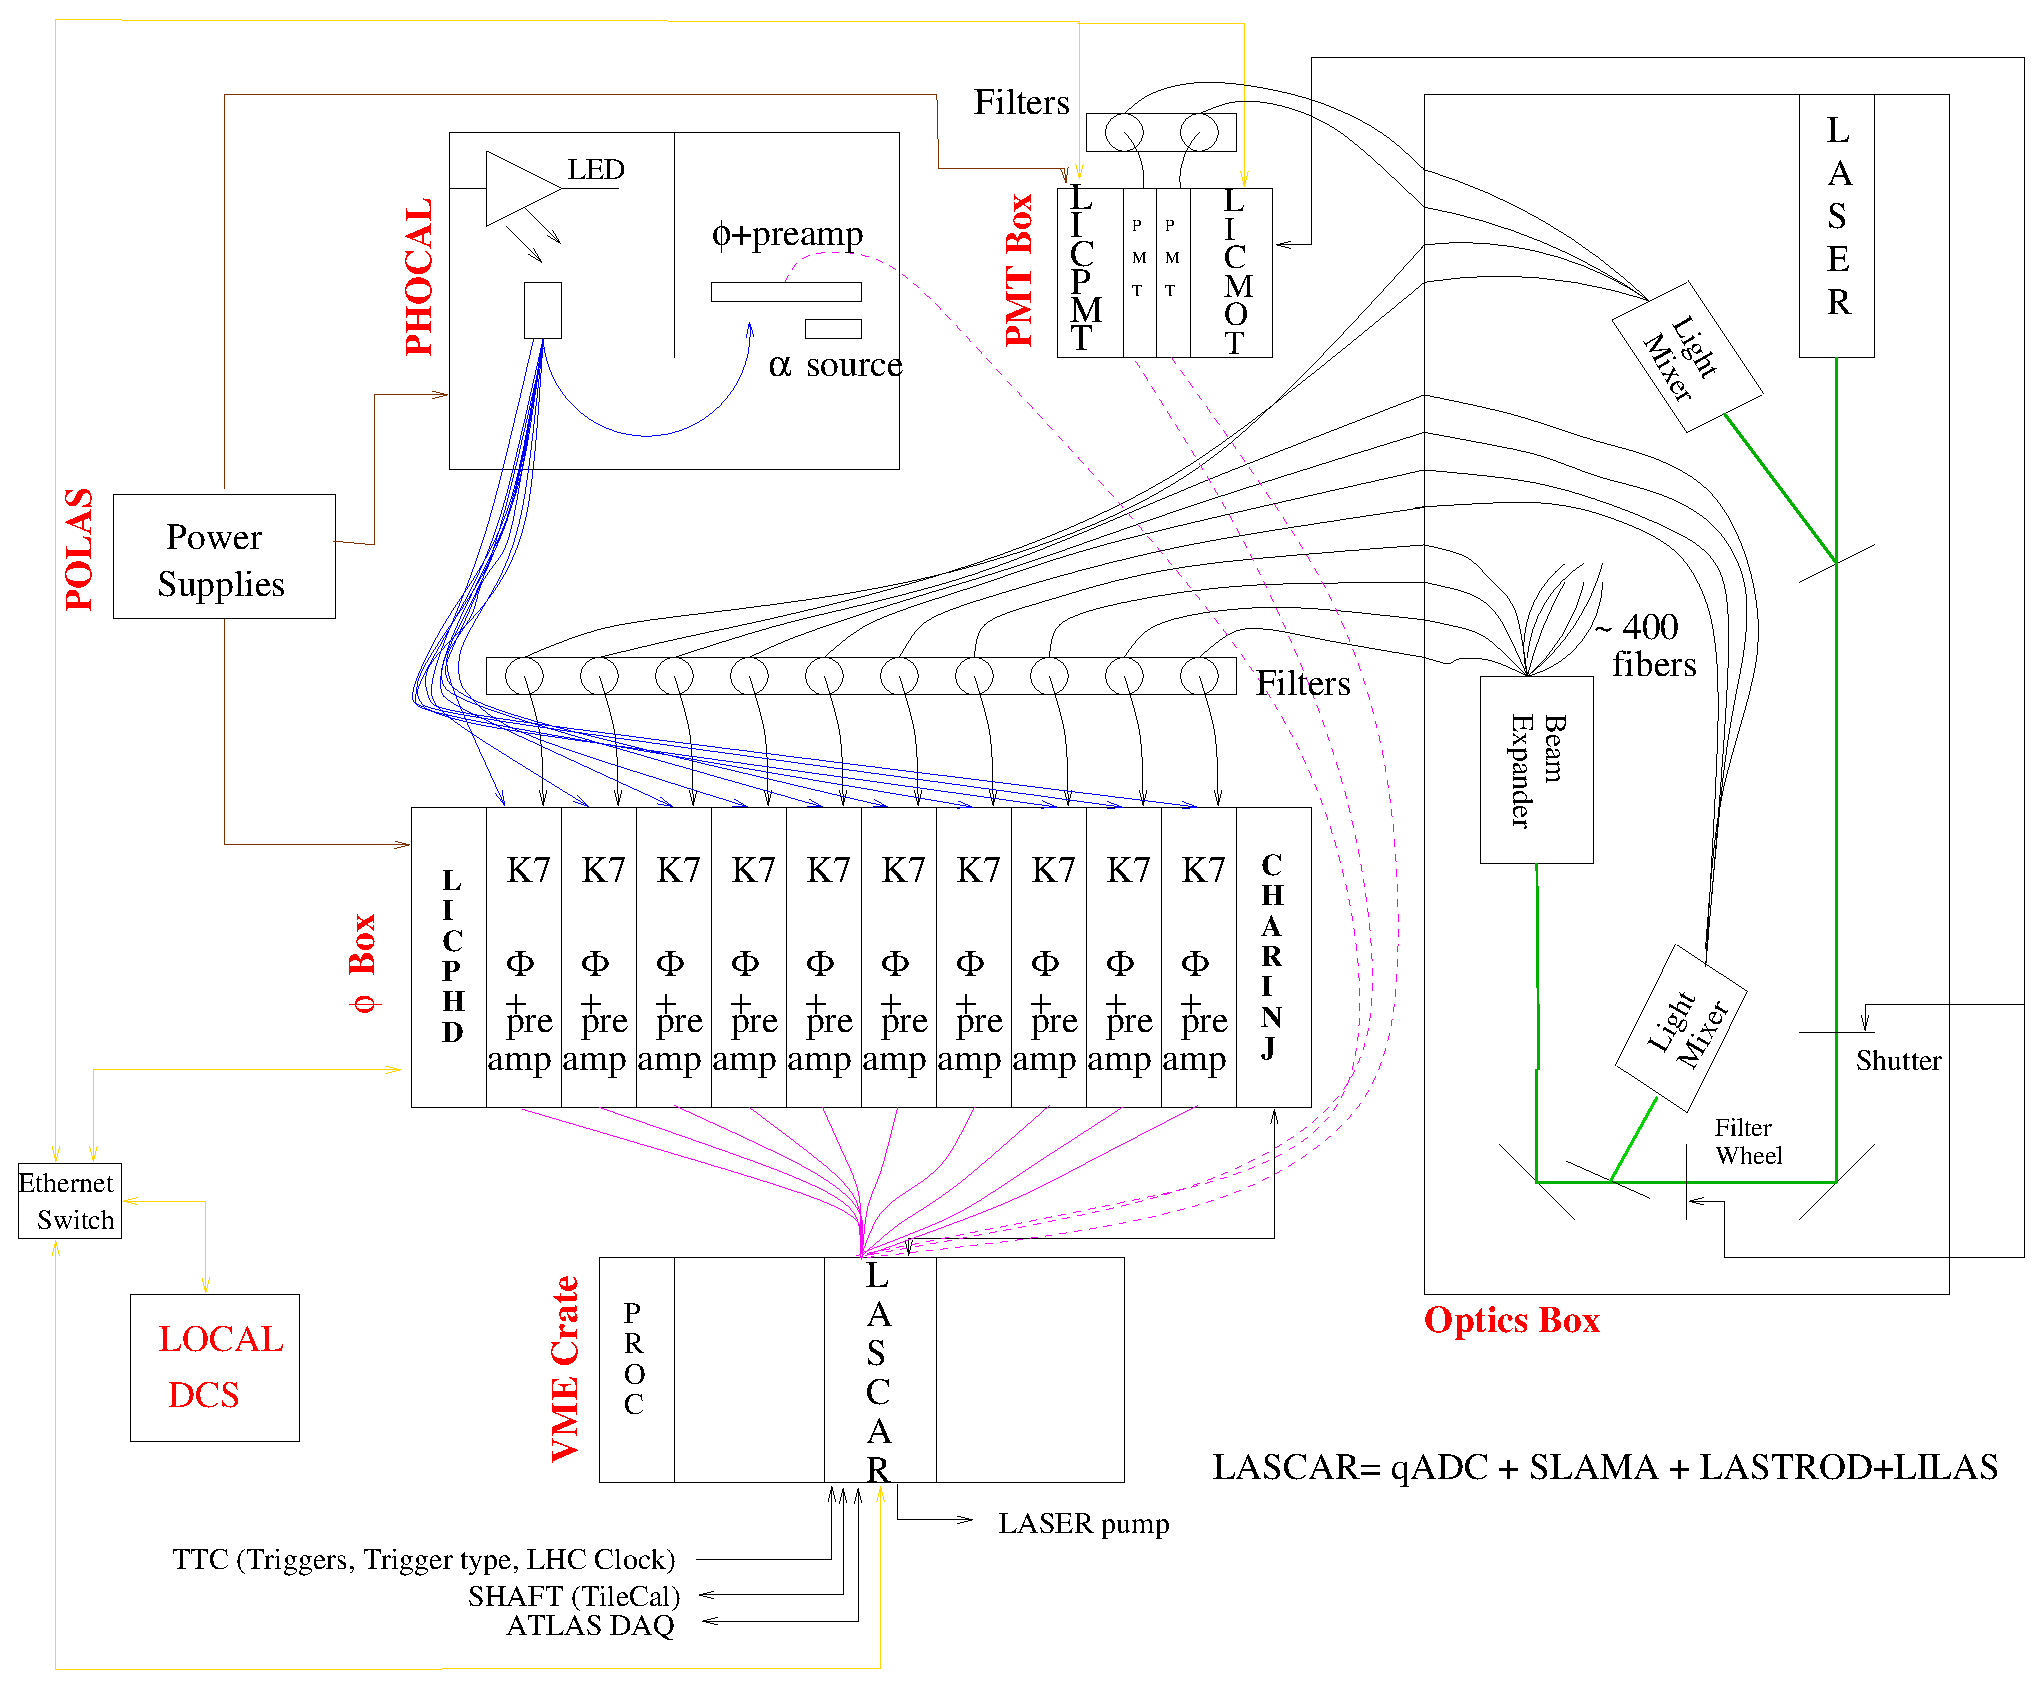
\includegraphics[width=9cm,height=11cm]{figures/LaserII_latest_latest.eps}
\caption{Scheme of the \lasii~system}\label{fig:laserscheme}
\end{figure}
\begin{itemize}
\item Optics box: at the output of the LASER head, the beam is transmitted through a beam expander (x2.5) and divided in two parts: one is sent to a light mixer that dispatches the light to seven optics fibers (3 are connected to photodiodes) while the other is reflected by a miror and trasmitted to a filter wheel. At the output of the filter wheel, the beam is splitted with one part sent to a light mixer (of the same kind as the first one, connected to three photodiodes) and the other part is sent to a beam expander which magnifies and dispatches the input light to a bundle of about 400 fibers. 4 fibers are connected to photodiodes while all others transmit the light to the modules of the TileCal.

\item Photodiode box: this box houses ten photodiodes (and their amplifier) receiving light from the optics box (LASER beam) or from \phocal~(LED signal). This box also contains two electronic boards, \licphd~and \charinjsplit.


\item \phocal: an internal calibration system named \phocal~(Photodiode Calibration) has been setup to monitor the stability of the ten photodiodes located in the photodiode box. It is composed of a LED emitting a signal in a light mixer that transmit the light to a set of 11 optics fibers, with 10 connected to the photodiode box, and one coupled to a reference photodiode. 
The stability of the ten photodiodes is performed through the monitoring of the LED signal received normalized to the magnitude measured by the reference photodiode. The stability of the reference photodiode is estimated thanks to a static radioactive source. 

\item PMT box: two PhotoMultiplier Tubes (PMTs) are used to trigger the acquisition when the LASER is flashing. The PMT box also contains two electronic cards, \licpmt~and \licmot.

\item Optical filters are used to attenuate the LASER signal transmitted to the photodiodes and the PMTs.

\item VME crate: two boards located in the VME crate are used to drive the \lasii~system: a VME Single Board Computer (SBC), and \lascar, that incorporates a charge analog-to-digital converter (qADC), and SLAMA, LASTROD and LILAS cards.

\item POwer LASer (\polas): power supplies of the \lasii~system. \polas~provides low voltages (+5V, -5V, $\pm$15V,+12 V, +24 V) to electronic boards.

\item Local DCS: a PC is used to collect slow-control information (such as temperatures, position of the filter wheel,...) from \licmot,\licpmt,\licphd~and \lascar~through ethernet connections.


\end{itemize}

\subsection{Electronics}

\subsubsection{Photodiode box}

\input photodiodebox.tex

\subsubsection{PMT box}

\input pmtbox.tex

\subsubsection{Internal calibration system : PHOCAL}

\input phocal.tex

\subsubsection{VME SBC}

\input sbc.tex

\subsubsection{LASCAR}

\input lascar.tex

\subsubsection{POLAS}

\input polas.tex

\subsection{Optics}

\subsubsection{Optics box}

\input opticsbox.tex

\subsubsection{Optical filters}

\input opticalfilters.tex

%\subsubsection{Optical path}
%\subsubsection{Light mixers and filter wheel}
%\subsubsection{Beam expander}

\subsection{DAQ}

\input daq.tex

\subsection{DCS}

\input dcs.tex


- description of the DCS: structure+data available+database access




%-------------------------------------------------------------------------------
\section{Conclusion}
\label{sec:conclusion}
%-------------------------------------------------------------------------------

Place your conclusion here.

\begin{comment}
%-------------------------------------------------------------------------------
\section*{Acknowledgements}
%-------------------------------------------------------------------------------

%% Acknowledgements for papers with collision data
% Version 19-Feb-2015

% Standard acknowledgements start here
%----------------------------------------------
We thank CERN for the very successful operation of the LHC, as well as the
support staff from our institutions without whom ATLAS could not be
operated efficiently.

We acknowledge the support of ANPCyT, Argentina; YerPhI, Armenia; ARC,
Australia; BMWFW and FWF, Austria; ANAS, Azerbaijan; SSTC, Belarus; CNPq and FAPESP,
Brazil; NSERC, NRC and CFI, Canada; CERN; CONICYT, Chile; CAS, MOST and NSFC,
China; COLCIENCIAS, Colombia; MSMT CR, MPO CR and VSC CR, Czech Republic;
DNRF, DNSRC and Lundbeck Foundation, Denmark; EPLANET, ERC and NSRF, European Union;
IN2P3-CNRS, CEA-DSM/IRFU, France; GNSF, Georgia; BMBF, DFG, HGF, MPG and AvH
Foundation, Germany; GSRT and NSRF, Greece; RGC, Hong Kong SAR, China; ISF, MINERVA, GIF, I-CORE and Benoziyo Center, Israel; INFN, Italy; MEXT and JSPS, Japan; CNRST, Morocco; FOM and NWO, Netherlands; BRF and RCN, Norway; MNiSW and NCN, Poland; GRICES and FCT, Portugal; MNE/IFA, Romania; MES of Russia and ROSATOM, Russian Federation; JINR; MSTD,
Serbia; MSSR, Slovakia; ARRS and MIZ\v{S}, Slovenia; DST/NRF, South Africa;
MINECO, Spain; SRC and Wallenberg Foundation, Sweden; SER, SNSF and Cantons of
Bern and Geneva, Switzerland; NSC, Taiwan; TAEK, Turkey; STFC, the Royal
Society and Leverhulme Trust, United Kingdom; DOE and NSF, United States of
America.

The crucial computing support from all WLCG partners is acknowledged
gratefully, in particular from CERN and the ATLAS Tier-1 facilities at
TRIUMF (Canada), NDGF (Denmark, Norway, Sweden), CC-IN2P3 (France),
KIT/GridKA (Germany), INFN-CNAF (Italy), NL-T1 (Netherlands), PIC (Spain),
ASGC (Taiwan), RAL (UK) and BNL (USA) and in the Tier-2 facilities
worldwide.
%----------------------------------------------



The \texttt{atlaslatex} package contains the acknowledgements that were valid 
at the time of the release you are using.
These can be found in the \texttt{acknowledgements} subdirectory.
When your ATLAS paper or PUB/CONF note is ready to be published,
download the latest set of acknowledgements from:\\
\url{https://twiki.cern.ch/twiki/bin/view/AtlasProtected/PubComAcknowledgements}

The supporting notes for the analysis should also contain a list of contributors.
This information should usually be included in \texttt{mydocument-metadata.tex}.
The list should be printed either here or before the table of contents.
\end{comment}

%-------------------------------------------------------------------------------
\clearpage
\appendix
\part*{Appendix}
\addcontentsline{toc}{part}{Appendix}

\input appendix.tex
%-------------------------------------------------------------------------------
\begin{comment}
In a paper, an appendix is used for technical details that would otherwise disturb the flow of the paper.
Such an appendix should be printed before the Bibliography.
\end{comment}

%-------------------------------------------------------------------------------
% If you use biblatex and either biber or bibtex to process the bibliography
% just say \printbibliography here
\printbibliography

% If you want to use the traditional BibTeX you need to use the syntax below.
%\bibliographystyle{bibtex/bst/atlasBibStyleWoTitle}
%\bibliography{LaserII_note,bibtex/bib/ATLAS}
%\input biblio.tex
%-------------------------------------------------------------------------------

%-------------------------------------------------------------------------------
% Print the list of contributors to the analysis
% The argument gives the fraction of the text width used for the names
%-------------------------------------------------------------------------------
\clearpage
\PrintAtlasContribute{0.30}

\begin{comment}
%-------------------------------------------------------------------------------
\clearpage
\appendix
\part*{Auxiliary material}
\addcontentsline{toc}{part}{Auxiliary material}
%-------------------------------------------------------------------------------

In an ATLAS paper, auxiliary plots and tables that are supposed to be made public 
should be collected in an appendix that has the title \enquote{Auxiliary material}.
This appendix should be printed after the Bibliography.
At the end of the paper approval procedure, this information can be split into a separate document
-- see \texttt{atlas-auxmat.tex}.

In an ATLAS note, use the appendices to include all the technical details of your work
that are relevant for the ATLAS Collaboration only (e.g.\ dataset details, software release used).
This information should be printed after the Bibliography.

\end{comment}

\end{document}
